% questions.tex —— 2018 年·天津卷·理科 · 题目内容片段（无答案）
% 由 tools/generate_projects.py 依来源总账自 2018/2018_数学真题_天津卷理_试题.md 生成，勿手改（改源 MD 后重跑）


\gkpart{数学}

\begin{gktip}
根据固定源印刷页1081—1082转录；出版者、版次、来源链与官方身份未核，固定源不含答案页。
\end{gktip}

\gkpart{一、选择题}

\begin{question}
\gkti{1}
设全集为 $\mathbb R$，集合 $A=\{x\mid 0<x<2\}$，$B=\{x\mid x\geqslant1\}$，则 $A\cap(\complement_{\mathbb R}B)=$（ ）。

(A) $\{x\mid 0<x\leqslant1\}$　(B) $\{x\mid 0<x<1\}$\\
(C) $\{x\mid 1\leqslant x<2\}$　(D) $\{x\mid 0<x<2\}$

\end{question}
\begin{question}
\gkti{2}
\Needspace{5\baselineskip}
设变量 $x,y$ 满足约束条件
\nopagebreak[4]
\[
\begin{cases}
x+y\leqslant5,\\
2x-y\leqslant4,\\
-x+y\leqslant1,\\
y\geqslant0,
\end{cases}
\]
则目标函数 $z=3x+5y$ 的最大值为（ ）。

(A) 6　(B) 19　(C) 21　(D) 45

\Needspace{0.4\textheight}
\end{question}
\begingroup
\renewenvironment{question}{\Needspace{0.5\textheight}}{}
\begin{question}
\gkti{3}

阅读如图所示的程序框图，运行相应的程序，若输入 $N$ 的值为 20，则输出 $T$ 的值为（ ）。
\nopagebreak[4]
\begin{center}% 2018 天津理科第3题程序框图（据固定源第1页重绘）
\begin{tikzpicture}[>=stealth, font=\small, node distance=5mm and 12mm]
  \tikzset{
    term/.style={draw, rounded corners=2pt, minimum width=12mm, minimum height=6mm, align=center},
    proc/.style={draw, minimum width=22mm, minimum height=7mm, align=center},
    test/.style={draw, diamond, aspect=2.7, inner sep=1pt, align=center},
    io/.style={draw, trapezium, trapezium left angle=70, trapezium right angle=110, minimum width=17mm, minimum height=6mm, align=center}
  }
  \node[term] (start) {开始};
  \node[io, below=of start] (input) {输入 $N$};
  \node[proc, below=of input] (init) {$i=2,\ T=0$};
  \node[test, below=of init, minimum width=29mm, minimum height=9mm] (div) {$\dfrac{N}{i}$ 是整数?};
  \node[proc, below=of div] (add) {$T=T+1$};
  \node[test, below=of add, minimum width=20mm, minimum height=8mm] (inc) {$i=i+1$};
  \node[test, below=of inc, minimum width=17mm, minimum height=7mm] (done) {$i\ge5$};
  \node[io, below=of done] (output) {输出 $T$};
  \node[term, below=of output] (end) {结束};
  \draw[->] (start)--(input);
  \draw[->] (input)--(init);
  \draw[->] (init)--(div);
  \draw[->] (div)--node[right]{是}(add);
  \draw[->] (add)--(inc);
  \draw[->] (div.east)--node[above]{否} ++(13mm,0)|-(inc.east);
  \draw[->] (inc)--(done);
  \draw[->] (done)--node[right]{是}(output);
  \draw[->] (output)--(end);
  \draw[->] (done.west)--node[above]{否} ++(-15mm,0)|-(div.west);
\end{tikzpicture}
\end{center}
\nopagebreak[4]
(A) 1　(B) 2　(C) 3　(D) 4

\end{question}
\endgroup
\begin{question}
\gkti{4}
设 $x\in\mathbb R$，则“$\left|x-\frac12\right|<\frac12$”是“$x^3<1$”的（ ）。

(A) 充分而不必要条件　(B) 必要而不充分条件\\
(C) 充要条件　(D) 既不充分也不必要条件

\end{question}
\begin{question}
\gkti{5}
已知 $a=\log_2 e$，$b=\ln2$，$c=\log_{1/2}\frac13$，则 $a,b,c$ 的大小关系为（ ）。

(A) $a>b>c$　(B) $b>a>c$　(C) $c>b>a$　(D) $c>a>b$

\end{question}
\begin{question}
\gkti{6}
将函数 $y=\sin\left(2x+\frac\pi5\right)$ 的图象向右平移 $\frac\pi{10}$ 个单位长度，所得图象对应的函数（ ）。

(A) 在区间 $\left[\frac{3\pi}4,\frac{5\pi}4\right]$ 上单调递增　(B) 在区间 $\left[\frac{3\pi}4,\pi\right]$ 上单调递减

(C) 在区间 $\left[\frac{5\pi}4,\frac{3\pi}2\right]$ 上单调递增　(D) 在区间 $\left[\frac{3\pi}2,2\pi\right]$ 上单调递减

\end{question}
\begin{question}
\gkti{7}
已知双曲线 $\frac{x^2}{a^2}-\frac{y^2}{b^2}=1\;(a>0,b>0)$ 的离心率为 2，过右焦点且垂直于 $x$ 轴的直线与双曲线交于 $A,B$ 两点。设 $A,B$ 到双曲线同一条渐近线的距离分别为 $d_1,d_2$，且 $d_1+d_2=6$，则双曲线的方程为（ ）。

(A) $\frac{x^2}{4}-\frac{y^2}{12}=1$　(B) $\frac{x^2}{12}-\frac{y^2}{4}=1$　(C) $\frac{x^2}{3}-\frac{y^2}{9}=1$　(D) $\frac{x^2}{9}-\frac{y^2}{3}=1$

\Needspace{0.4\textheight}
\end{question}
\begin{question}
\gkti{8}
如图，在平面四边形 $ABCD$ 中，$AB\perp BC$，$AD\perp CD$，$\angle BAD=120^\circ$，$AB=AD=1$。若点 $E$ 为边 $CD$ 上的动点，则 $\overrightarrow{AE}\cdot\overrightarrow{BE}$ 的最小值为（ ）。
\nopagebreak[4]
\begin{center}% 2018 天津理科第8题几何示意图（据固定源第1页重绘）
\begin{tikzpicture}[font=\small, line cap=round, line join=round]
  % AB=AD=1, angle BAD=120 degrees; perpendicularities determine C.
  \coordinate (A) at (0,0);
  \coordinate (B) at (1.8,0);
  \coordinate (D) at (-0.9,1.559);
  \coordinate (C) at (1.8,3.118);
  \coordinate (E) at ($(D)!0.48!(C)$);
  \draw (A)--(D)--(C)--(B)--(A);
  \draw (A)--(E)--(B);
  \node[below] at (A) {$A$};
  \node[right] at (B) {$B$};
  \node[above] at (C) {$C$};
  \node[left] at (D) {$D$};
  \node[left] at (E) {$E$};
\end{tikzpicture}
\end{center}
\nopagebreak[4]
(A) $\frac{21}{16}$　(B) $\frac32$　(C) $\frac{25}{16}$　(D) $3$

\end{question}
\gkpart{二、填空题}

\begin{question}
\gkti{9}
$i$ 是虚数单位，复数 $\frac{6+7i}{1+2i}=\underline{\qquad\qquad}$。

\end{question}
\begin{question}
\gkti{10}
在 $\left(x-\frac{1}{2\sqrt{x}}\right)^5$ 的展开式中，$x^2$ 的系数为 $\underline{\qquad\qquad}$。

\Needspace{0.4\textheight}
\end{question}
\begin{question}
\gkti{11}
已知正方体 $ABCD-A_1B_1C_1D_1$ 的棱长为 1，除面 $ABCD$ 外，该正方体其余各面的中心分别为点 $E,F,G,H,M$（如图），则四棱锥 $M-EFGH$ 的体积为 $\underline{\qquad\qquad}$。
\nopagebreak[4]
\begin{center}% 2018 天津理科第11题：正方体五个面的中心及四棱锥示意图。
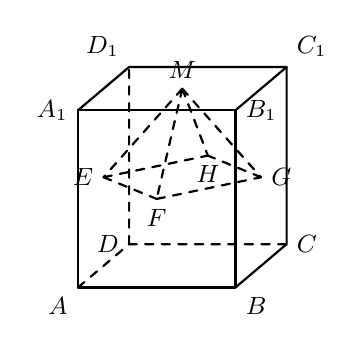
\begin{tikzpicture}[line cap=round,line join=round,thick,every node/.style={font=\small}]
  % Oblique projection of the unit cube; ABCD is the bottom face.
  \coordinate (A) at (0,0);
  \coordinate (B) at (2,0);
  \coordinate (C) at (2.65,.55);
  \coordinate (D) at (.65,.55);
  \coordinate (A1) at (0,2.25);
  \coordinate (B1) at (2,2.25);
  \coordinate (C1) at (2.65,2.8);
  \coordinate (D1) at (.65,2.8);
  % Cube edges: hidden rear-left edges are dashed.
  \draw (A)--(B)--(B1)--(A1)--cycle;
  \draw (A1)--(D1)--(C1)--(B1);
  \draw (B)--(C)--(C1);
  \draw[dashed] (A)--(D)--(C) (D)--(D1);
  % Centers of the top, left, back, right and front faces (ABCD excluded).
  \coordinate (M) at (1.325,2.525);
  \coordinate (E) at (.325,1.4);
  \coordinate (F) at (1,1.125);
  \coordinate (G) at (2.325,1.4);
  \coordinate (H) at (1.65,1.675);
  % The source depicts the internal pyramid construction with dashed lines.
  \draw[dashed] (M)--(E) (M)--(F) (M)--(G) (M)--(H);
  \draw[dashed] (E)--(F) (E)--(H) (F)--(G) (G)--(H);
  \node[below left] at (A) {$A$};
  \node[below right] at (B) {$B$};
  \node[right] at (C) {$C$};
  \node[left] at (D) {$D$};
  \node[left] at (A1) {$A_1$};
  \node[right] at (B1) {$B_1$};
  \node[above right] at (C1) {$C_1$};
  \node[above left] at (D1) {$D_1$};
  \node[above] at (M) {$M$};
  \node[left] at (E) {$E$};
  \node[below] at (F) {$F$};
  \node[right] at (G) {$G$};
  \node[below] at (H) {$H$};
\end{tikzpicture}
\end{center}
\nopagebreak[4]
\end{question}
\begin{question}
\gkti{12}
\Needspace{5\baselineskip}
已知圆 $x^2+y^2-2x=0$ 的圆心为 $C$，直线
\nopagebreak[4]
\[
\begin{cases}
x=-1+\dfrac{\sqrt2}{2}t,\\
y=3-\dfrac{\sqrt2}{2}t,
\end{cases}\qquad(t\text{ \text{为参数}})
\]
与该圆相交于 $A,B$ 两点，则 $\triangle ABC$ 的面积为 $\underline{\qquad\qquad}$。

\end{question}
\begin{question}
\gkti{13}
已知 $a,b\in\mathbb R$，且 $a-3b+6=0$，则 $2^a+\frac1{8^b}$ 的最小值为 $\underline{\qquad\qquad}$。

\end{question}
\begin{question}
\gkti{14}
\Needspace{5\baselineskip}
已知 $a>0$，函数
\nopagebreak[4]
\[
f(x)=\begin{cases}
x^2+2ax+a,&x\leqslant0,\\
-x^2+2ax-2a,&x>0,
\end{cases}
\]
若关于 $x$ 的方程 $f(x)=ax$ 恰有 2 个互异的实数解，则 $a$ 的取值范围是 $\underline{\qquad\qquad}$。

\end{question}
\gkpart{三、解答题}

\begin{question}
\gkti{15}
\Needspace{5\baselineskip}
在 $\triangle ABC$ 中，内角 $A,B,C$ 所对的边分别为 $a,b,c$。已知
\nopagebreak[4]
\[
b\sin A=a\cos\left(B-\frac\pi6\right).
\]

(1) 求角 $B$ 的大小；

(2) 设 $a=2,c=3$，求 $b$ 和 $\sin(2A-B)$ 的值。

\end{question}
\begin{question}
\gkti{16}
已知某单位甲、乙、丙三个部门的员工人数分别为 24、16、16。现采用分层抽样的方法从中抽取 7 人，进行睡眠时间的调查。

(1) 应从甲、乙、丙三个部门的员工中分别抽取多少人？

(2) 若抽出的 7 人中有 4 人睡眠不足，3 人睡眠充足，现从这 7 人中随机抽取 3 人做进一步的身体检查。

① 用 $X$ 表示抽取的 3 人中睡眠不足的员工人数，求随机变量 $X$ 的分布列与数学期望；

② 设 $A$ 为事件“抽取的 3 人中，既有睡眠充足的员工，也有睡眠不足的员工”，求事件 $A$ 发生的概率。

\Needspace{0.4\textheight}
\end{question}
\begin{question}
\gkti{17}
如图，$AD\parallel BC$ 且 $AD=2BC$，$AD\perp CD$，$EG\parallel AD$ 且 $EG=AD$，$CD\parallel FG$ 且 $CD=2FG$，$DG\perp$ 平面 $ABCD$，$DA=DC=DG=2$。

(1) 若 $M$ 为 $CF$ 的中点，$N$ 为 $EG$ 的中点，求证：$MN\parallel$ 平面 $CDE$；

(2) 求二面角 $E-BC-F$ 的正弦值；

(3) 若点 $P$ 在线段 $DG$ 上，且直线 $BP$ 与平面 $ADGE$ 所成的角为 $60^\circ$，求线段 $DP$ 的长。
\nopagebreak[4]
\begin{center}% 2018 天津理科第17题：空间几何示意，按原卷线型描绘。
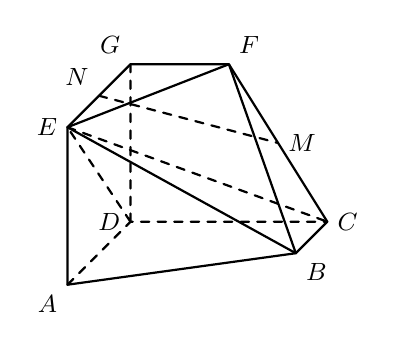
\begin{tikzpicture}[line cap=round,line join=round,thick,every node/.style={font=\small}]
  \coordinate (A) at (0,0);
  \coordinate (D) at (.8,.8);
  \coordinate (C) at (3.3,.8);
  \coordinate (B) at (2.9,.4);
  \coordinate (E) at (0,2);
  \coordinate (G) at (.8,2.8);
  \coordinate (F) at (2.05,2.8);
  % Solid visible outer edges.
  \draw (A)--(B)--(C)--(F)--(G)--(E)--(A);
  \draw (E)--(F) (F)--(B) (E)--(B);
  % Midpoints shown on the upper/rear edges.
  \coordinate (N) at (.4,2.4);
  \coordinate (M) at (2.675,1.8);
  % Rear/under edges and construction lines hidden in the source.
  \draw[dashed] (A)--(D)--(C) (D)--(G) (D)--(E);
  \draw[dashed] (E)--(C) (N)--(M);
  \node[below left] at (A) {$A$};
  \node[below right] at (B) {$B$};
  \node[right] at (C) {$C$};
  \node[left] at (D) {$D$};
  \node[left] at (E) {$E$};
  \node[above left] at (G) {$G$};
  \node[above right] at (F) {$F$};
  \node[above left] at (N) {$N$};
  \node[right] at (M) {$M$};
\end{tikzpicture}
\end{center}
\nopagebreak[4]
\end{question}
\begin{question}
\gkti{18}
设 $\{a_n\}$ 是等比数列，公比大于 0，其前 $n$ 项和为 $S_n\;(n\in\mathbb N^*)$，$\{b_n\}$ 是等差数列。

\Needspace{5\baselineskip}
已知
\nopagebreak[4]
\[
a_1=1,\quad a_3=a_2+2,\quad a_4=b_3+b_5,\quad a_5=b_4+2b_6.
\]

(1) 求 $\{a_n\}$ 和 $\{b_n\}$ 的通项公式；

(2) 设数列 $\{S_n\}$ 的前 $n$ 项和为 $T_n\;(n\in\mathbb N^*)$。

① 求 $T_n$；

\Needspace{5\baselineskip}
② 证明
\nopagebreak[4]
\[
\sum_{k=1}^{n}\frac{(T_k+b_{k+2})b_k}{(k+1)(k+2)}=\frac{2^{n+2}}{n+2}-2\qquad(n\in\mathbb N^*).
\]

\end{question}
\begin{question}
\gkti{19}
设椭圆 $\frac{x^2}{a^2}+\frac{y^2}{b^2}=1\;(a>b>0)$ 的左焦点为 $F$，上顶点为 $B$。已知椭圆的离心率为 $\frac{\sqrt5}{3}$，点 $A$ 的坐标为 $(b,0)$，且 $|FB|\cdot|AB|=6\sqrt2$。

(1) 求椭圆的方程；

\Needspace{5\baselineskip}
(2) 设直线 $l:y=kx\;(k>0)$ 与椭圆在第一象限的交点为 $P$，且 $l$ 与直线 $AB$ 交于点 $Q$。若
\nopagebreak[4]
\[
\frac{|AQ|}{|PQ|}=\frac{5\sqrt2}{4}\sin\angle AOQ\qquad(O\text{ \text{为原点}}),
\]
求 $k$ 的值。

\end{question}
\begin{question}
\gkti{20}
已知函数 $f(x)=a^x$，$g(x)=\log_a x$，其中 $a>1$。

(1) 求函数 $h(x)=f(x)-x\ln a$ 的单调区间；

\Needspace{5\baselineskip}
(2) 若曲线 $y=f(x)$ 在点 $(x_1,f(x_1))$ 处的切线与曲线 $y=g(x)$ 在点 $(x_2,g(x_2))$ 处的切线平行，证明
\nopagebreak[4]
\[
x_1+g(x_2)=-\frac{2\ln\ln a}{\ln a};
\]

(3) 证明当 $a\geqslant e^{1/e}$ 时，存在直线 $l$，使 $l$ 是曲线 $y=f(x)$ 的切线，也是曲线 $y=g(x)$ 的切线。

\end{question}